\chapter{ Information Transfer Estimation on Large Data} \label{Chapter:PyIF}
\blfootnote{
	This chapter contains material from the following publication: 
	\nobibliography{thesisbib}
	\begin{itemize}
		\item\bibentry{PyIF}
	\end{itemize}
}

\section{Introduction}

%\RC{I don't get second sentence. Is canonical systems something meant like social media or neuroscience, or do you mean the last three are canonical systems?}

Transfer entropy (TE) is an information measure that quantifies the transfer of information between processes evolving in time (see Chapter \ref{sec:InformationTheory}). Transfer entropy has many potential applications in  neuroscience, social media, and financial markets. Prior TE work concerning financial applications has typically used long windows in their research. For example, \cite{Kantz} measured information transfer between two financial time series (the DAX stock index and the Dow Jones) to determine to what extent one index determined the other's behavior. The data used by \cite{Kantz} sampled data every minute between May 2000 and June 2001; after cleaning the data, 63,867 observations were used in \cite{Kantz}'s study.  More recently \cite{Sandoval} used daily price data from 2003 to 2012 to detect causal relationships between 197 largest firms (globally) with Transfer Entropy.

Given the assumption in Chapter \ref{IFinFM} that information is reflected in price and in an efficient market changes rapidly (if not instantaneously), then slower frequencies of observations (or long time windows) such as monthly, daily, hourly, or even by the minute may be insufficient in capturing the price change process.  Given that we may not capture the entire price change process with long time windows between each observation, we examine price change with shorter windows.  However, shorter time windows will have a finer resolution of data, requiring more observations in a dataset. 
%To illustrate this I provide an example of the amount observations that  increase given the time scale in Figure \ref{fig:FreqObs}. 

In Figure \ref{fig:FreqObs}, we present the number of observations for a univariate dataset over 30 days for varying frequency size.  If the frequency of observations (time windows) in 30 days is daily,  there are 30 observations in the dataset.  If the time windows are hourly, we can expect 720 observations in 30 days, and if the time window between observations occurs on a minute level, then we have 43,200 observations.  If we continue these calculations down to the 1-second level, then there are 2,592,000 observations in a 30-day window.  Following this trend, we find that existing open-source, TE computation implementations are not suited to estimate information flow for datasets with large numbers of observations.  Given the need to examine information transfers over finer time resolutions, we propose a new, open-source, software implementation to estimate TE for large datasets.

\section{Estimating Transfer Entropy} \label{intro:estimateTE}

Prior research has developed a few approaches for estimating TE. There is a requirement to specify the following parameter choices: the time between periods, length of the time series, number of past observations that inform the future observations, and the direction of information transfer in the approaches. The correct approach depends on the underlying data. There are many techniques for estimating mutual information. \cite{EstimatingTE} explored the utility of different methods for mutual information estimation, and many of the methods are applicable to estimate TE.

\subsection{Kraskov Estimator} \label{intro:Kraskov}


\cite{kraskovEstimator} outlined a widely used method  to estimate Transfer Entropy by using a k-nearest neighbor algorithm.  Note, to estimate entropy:

\begin{equation}
\hat{H}(X) = - \frac{1}{n} \sum^n_{i=1} ln (\hat{p}(x_i)) 
\end{equation}

\noindent Kraskov et al. expanded this definition to estimate entropy to:

\setlength{\arraycolsep}{0.0em}
\begin{eqnarray}
\hat{H}(X) = - \frac{1}{n} \sum^n_{i=1} \psi(n_x(i)) - \frac{1}{k} + \psi(n) + ln (c_{d_x}) + \nonumber\\
 \frac{d_x}{n} \sum^n_{i=1} ln (\epsilon(i))
\end{eqnarray}
\setlength{\arraycolsep}{1pt}

%\begin{equation} \hat{H}(X) = - \frac{1}{n} \sum^n_{i=1} \psi(n_x(i)) - \frac{1}{k} + \psi(n) + ln (c_{d_x}) + \frac{d_x}{n} \sum^n_{i=1} ln (\epsilon(i)) \end{equation},
\noindent where n are the number of data points, k is a parameter to select the number of nearest neighbors,  \(d_x\) is the dimension of x, and \(c_{d_x}\) is the volume of the \(d_x\)-dimensional unit ball. For two random variables X and Y, let \( \frac{\epsilon(i)}{2} \) be the distance between (\(x_i,y_i\)) and it's k\textsuperscript{th} neighbor be denoted by (\(kx_i,ky_i\)). Let \(\frac{\epsilon_x(i)}{2}\) and  \(\frac{\epsilon_y(i)}{2}\) be defined as \( ||x_i-kx_i ||\) and \( ||y_i-ky_i || \) respectively where,  \(||\ \ldots\ ||\) is the max-norm distance between the \(i^{th}\) data point and \(k^{th}\) nearest neighbor data point.  \(n_x(i)\) is the number of points \(x_j\) such that \(||x_i - x_j  || \leq \epsilon_x(i)/2\), \(\psi(x)\) is the digamma function where:

\begin{equation}
\psi(x) = \Gamma(x)^{-1} \frac{d\Gamma(x)} {dx}
\end{equation}

\noindent and  \(\Gamma(x)\) is the ordinary gamma function. Lastly \(\psi(1) = -C\) where \(C=0.5772156649\) and is the Euler-Mascheroni constant. %To estimate the entropy for the random variable Y, \(Y\) can be substituted into \(\hat{H}(X)\).

To estimate Joint entropy between X and Y: 

\setlength{\arraycolsep}{0.0em}
\begin{eqnarray}
\hat{H}(X,Y) = - \psi(k) - \frac{1}{k} + \psi(n) + ln(c_{d_x} c_{d_y})  +  \nonumber\\
\frac{d_x + d_y}{n} \sum^n_i ln(\epsilon(i))
\end{eqnarray}
\setlength{\arraycolsep}{1pt}

%\begin{equation}\hat{H}(X,Y) = - \psi(k) - \frac{1}{k} + \psi(n) + ln(c_{d_x} c_{d_y})  + \frac{d_x + d_y}{n} \sum^n_i ln(\epsilon(i))\end{equation}

\noindent where \(d_y\) is the dimension of \(y\), and \(c_{d_y}\) is the column of the \(d_y\)-dimensional unit ball. Using \(\hat{H}(X), \hat{H}(Y),\) and \(\hat{H}(X,Y)\), Kraskov shows that mutual information can be estimated as:

\begin{equation}
\label{KraskovEquation}
\hat{I}(X,Y) = \psi(k) - \frac{1}{k} - \frac{1}{n}  \sum_{i=1}^n [\psi(n_x(i)) + \psi(n_y(i))] + \psi(n)
\end{equation}

\noindent where \(n_y(i)\) is the number of points \(y_j\) such that \(|| y_i - y_j || \leq \frac{\epsilon_y(i)}{2} \).

%HERE
The basic idea of mutual information estimation with the Kraskov's estimator is for each observation \(i\) to count the number \(n_x(i)\) (or \(n_y(i)\)) of points less than the distance between \(x_i\) (or \(y_i\)) and the \(k^{th}\) neighbor. The distance or \(\epsilon(i)\) fluctuates for each observation, consequently, \(n_x(i)\) and \(n_y(i)\) fluctuate. The counts are averaged over all observations, which results in mutual information as defined in Equation \ref{KraskovEquation}.


To estimate TE with Kraskov's estimator, recall from Equation \ref{eq:TE-MI-Diff} that TE is expressed as the difference between two mutual information computations. To estimate TE with Equation \ref{eq:TE-MI-Diff}, the first mutual information is between \(Y\)'s future value, \(Y\)'s lagged values, and the  \(X\)'s lagged values. The second mutual information is the mutual information between X and its lagged values. The difference between the first and second mutual information provide the TE. With an embedding of \(1\), TE can be estimated: 

\setlength{\arraycolsep}{0.0em}
\begin{eqnarray}
TE_{Y \rightarrow X} =  \left[  \psi(k) - \frac{1}{k} - \frac{1}{n}  \sum_{i=1}^n [ \psi(n_{xy}^{(t)}(i)) + \psi(n_{xy}^{(t-1)}(i) ) ] + \psi(n) \right]   -  \nonumber\\
\left[  \psi(k) - \frac{1}{k} - \frac{1}{n}  \sum_{i=1}^n [ \psi(n_{x}^{(t)}(i)) + \psi(n_{x}^{(t-1)}(i) ) ] + \psi(n) \right]
\label{eq:TE-EST}
\end{eqnarray}
\setlength{\arraycolsep}{1pt}

\noindent  Here \(n_{xy}\) is the number of points \(y_j\) such that \(||y_i - y_j  || \leq \epsilon_y(i)/2\) and \(||x_i - y_j  || \leq \epsilon_y(i)/2\).

\subsection{Additional Estimators}
\cite{EstimatingTE} also explored the utility of Kernel Density Estimation, Edgeworth approximation of differential entropy to calculate Mutual Information, and adaptive partitioning of the XY plane to estimate the joint probability density, which can estimate mutual information. Ultimately \cite{EstimatingTE} found that a KDE estimator and Kraskov estimator outperform other methods for their ability to capture the dependence structure of random processes. \cite{JeffTE} examined the properties of the Kraskov estimator between equities and their underlying options. They ultimately provided evidence that incorrect parameter choices lead to smaller TE estimates and that Kraskov's method has a downward bias indicating that it underestimates information transfer. Nevertheless, it is relatively insensitive to parameter selection. 


\section{PyIF}

PyIF \footnote{PyIF can freely be downloaded from: \url{https://github.com/lcdm-uiuc/PyIF}} is our proposed, open-source software implementation to estimate bivariate TE on large data.  PyIF currently only supports using the Kraskov estimator to estimate TE.  PyIF utilizes recent advancements in hardware to parallelize \& optimize operations across CPUs and CUDA compatible GPUs (see  \cite{CUDA}).  Given the iterative nature of Equation \ref{eq:TE-EST} it is possible to speed up the estimation by performing computations in parallel. In particular, we focus our efforts on the parallelization \& optimization across operations to obtain \(n_x\)  \& \(n_{xy}\) in Equation \ref{eq:TE-EST} faster.

%\RC{Define CPU and GPU?}

% more here on how we do this?

PyIF is a Python implementation that utilizes five well-known and actively supported Python libraries: SciPy (see \cite{scipy}),  NumPy (see \cite{numpy}), scikit-learn (see \cite{scikit-learn}),  nose (see \cite{nose}), and numba (see \cite{numba}).  SciPy is an open-source Python library used for a variety of STEM applications.  NumPy is a part of SciPy's ecosystem and is an open-source package that provides convenient ways to perform matrix manipulations and useful linear algebra capabilities.  Scikit-learn is a popular open-source library for machine learning, and nose is another open-source library that is useful for testing code to ensure that it will produce the correct outcome.  Lastly, numba is a Python tool that can compile Python code to execute multicore CPUs and CUDA-capable GPUs.

%HERE IN GRAMMARLY

PyIF's interface requires one to supply \(X\) and \(Y\), two NumPy arrays with \(N\)x1 dimensions.  PyIF supports optional arguments such as \(k\), which controls the number of neighbors used in KD-tree nearest neighbor searches,  \(embedding\), which controls how many lagged periods are in the transfer entropy computation, and a boolean argument \(GPU\) , which allows one to use a CUDA compatible GPU for transfer entropy estimation.  Lastly, \(safetyCheck\) is a boolean argument that can check for duplicate rows in the dataset. This boolean argument helps prevent a more subtle error when multiple data points in a bivariate dataset have identical coordinates. For duplicate observations, several points have an identical distance to a query point during k nearest neighbors search, which violates assumptions of the Kraskov estimator. A solution used in practice and that we recommend is to add a small amount of noise to the dataset to avoid this error.


\section{Comparative Analysis} \label{PyIF:CA}

We compare PyIF's ability to estimate Transfer Entropy against existing implementations with respect to computational performance. We present all of the data and code used to estimate TE for all implementations \footnote{The data and code can freely be downloaded from: \\  \url{https://github.com/lcdm-uiuc/Publications/tree/master/2020\_Ikegwu\_Traguer\_McMullin\_Brunner}}. Each implementation in this comparative analysis estimates TE on four simulated bivariate datasets of different sizes. The estimated TE values are roughly the same for each implementation, and we forgo comparing the actual values since this is random simulated data. Thus, we assume that there is relatively little to no information transfer between the random processes. We run each of the implementations (excluding Transfer Entropy Toolbox)  on nano, a cluster of eight SuperMicro servers with Intel Haswell/Broadwell CPUs and NVIDIA Tesla P100/V100 GPUs hosted by the National Center of Super Computing Applications at the University of Illinois at Urbana-Champaign. We used one node containing two E5-2620 v3 Intel Xeon CPUs and two NVIDIA P100 GPUs with 3584 cores.  We refer to this as the first analysis.

We conduct the same analysis on different hardware to compare PyIF to Transfer Entropy toolbox because of MATLAB licensing issues with the National Center of Super Computing Applications. We use an Engineering Workstation with an Intel Xeon Processor E5-2680 v4  hosted by Engineering IT shared services at the University of Illinois at Urbana-Champaign. We use a single CPU core and up to 16GB of RAM to estimate TE with Transfer Entropy toolbox and PyIF. This workstation does not offer CUDA compatible GPUs for either PyIF or Transfer Entropy Toolbox, so we forgo comparing the GPU implementations. This workstation has a CPU time limit of 60 minutes, meaning that if any process uses 100\% of a CPU core for more than 60 minutes, the process is terminated. We refer to this as the second analysis.

\subsection{IDTxl}
The first implementation that we compare PyIF to is the Information Dynamics Toolkit xl (IDTxl). IDTxl is an open-source Python toolbox for network inference (see \cite{IDTxl}). Currently, IDTxl relies on NumPy,  SciPy, CFFI (which is another open source library that provides a C interface for Python code; see \cite{cffi}),  H5py which is a Python package that is used to interface with HDF5 binary data format (see \cite{hdf5}),  JPype (see \cite{jpype}) which is a Python module that provides a Java interface for Python code, and Java JDK, which is a developer kit to develop Java applications and applets.  IDTxl has additional functionality besides estimating TE; however, we only use IDTxl's capability to estimate TE on a bi-variate dataset.


\subsection{TransEnt}
TransEnt is a R package that estimates transfer entropy (see \cite{TransEnt}). Currently, TransEnt relies on Rcpp, which acts as an interface to C++ from R. TransEnt also relies on a C++ library called Approximate Nearest Neighbors (ANN; see \cite{ANN}), which performs exact and approximate nearest neighbor searches. Currently, the package is removed from CRAN. However, this software can be used and installed from \cite{TransEnt}'s Github repository~\footnote{\cite{TransEnt}'s Github Repo: \url{https://github.com/Healthcast/TransEnt}}.

\subsection{RTransferEntropy}
RTransferEntropy is a R package that estimates transfer entropy between two time-series \cite{RTransferEntropy}. Currently, the RTransferEntropy package relies on Rcpp, and the future package supports performing computations in parallel to decrease the wall time. We include both the parallel implementation of RTransferEntropy and the default implementation for completeness in the results.


\subsection{Transfer Entropy Toolbox}

Transfer Entropy Toolbox  is an open-source MATLAB toolbox for transfer entropy estimation (see \cite{TransferEntropyToolbox}). This code's dependencies include: the Statistics \& Machine Learning toolbox, which provides functions to analyze and model data; the FieldTrip toolbox, which is used for EEG, iEEG, MEG, and NIRS analysis; the parallel computing toolbox, which performs parallel computations of multicore CPUs and GPUs; the signal processing toolbox, which provides functions to analyze, preprocess, and extract features from sampled signals; and the TSTOOL toolbox, which is a toolbox for nonlinear time series analysis. TSTOOL no longer exists and cannot be download from its official homepage \footnote{\url{http://www.dpi.physik.uni-goettingen.de/tstool/}}. Nevertheless, the Transfer Entropy toolbox developers include pre-compiled mex files of TSTOOL that will work with this implementation. At the time of writing,  Transfer Entropy toolbox's last update was in the year 2017.

\subsection{Data}

We create four bivariate datasets for this comparative analysis. Each dataset contains two time series with randomly generated values between 0 and 1. The first dataset contains 1000 observations, the second dataset contains 10,000 observations, the third dataset contains 100,000 observations, and the fourth dataset contains 1,000,000 observations.  We used the seed number  \(23\) for the pseudo-random number generator for reproducibility. We will refer to the first dataset, second dataset, third dataset, and fourth dataset as the micro dataset, small dataset, medium dataset, and the large dataset respectively.

\section{Results}

We report the results for Analysis 1 in Tables \ref{tab:MicroResults1},  \ref{tab:SmallResults1}, \ref{tab:MediumResults1}, and \ref{tab:LargeResults1}.  Each table contains the wall time to estimate TE using the previously deinfed implementations on the different data sets described in section \ref{PyIF:CA}.  The higher the wall time, the longer it took for the specific implementation to estimate TE.  The number in the relative performance column indicates how many times slower (or faster) PyIF (CPU) is to a particular implementation.  After estimating TE by using all of the implementations outlined in the comparative analysis section, we found that PyIF scales better on larger data.  

Excluding the TransEnt implementation, the CPU implementation of PyIF (or PyIF (CPU)) takes less time to estimate TransferEntropy than all other implementations. The R package TransEnt has a better performance in terms of speed than PyIF (CPU) for the micro dataset and the small dataset. However, PyIF (CPU) can estimate transfer entropy in less time then all other implementations for the medium dataset and large dataset. PyIF (GPU) outperforms PyIF (CPU) for the small, medium, and large datasets. Figure \ref{TE-walltime} visualizes this explanation. We suspect that the optimizations performed by Numba contribute to PyIF having a larger wall time than TransEnt on the micro and small datasets.

The results for Analysis 2 are in Table ~\ref{DataTable-MATLAB}.  Although the Transfer Entropy Toolbox exceeds the CPU time limit for the large dataset, the results show that PyIF can scale better than Transfer Entropy Toolbox for the other three datasets. PyIF's wall times are less than Transfer Entropy toolbox's wall times, excluding the Micro Dataset.  Figure \ref{TE-walltime2} visualizes this result.


\section{Conclusion}

We address an important issue regarding large datasets with respect to the estimation of bi-variate TE. We introduce a fast solution to estimate TE with a small number of software dependencies. On large data, our implementation, PyIF, is up to 1072 times faster utilizing GPUs and up to 181 times faster utilizing CPUs than existing implementations that estimate bi-variate TE.  PyIF is also open sourced and publicly available on Github for anyone to use.  For future work, we plan to improve the existing code base to increase the computational performance of PyIF even further. We plan to implement additional estimators outlined in section  \ref{intro:estimateTE} to estimate bi-variate TE. This boost in computational performance will enable researchers to estimate bi-variate TE much faster for various research applications. In particular, PyIF will allow us to estimate information transfer between firms with small windows in a reasonable amount of time.

%\section*{Acknowledgments}
%This work was partially funded by the Graduate College Fellowship program at the University of Illinois. This work utilizes resources provided by the Innovative Systems Laboratory at the National Center for Supercomputing Applications at the University of Illinois at Urbana-Champaign. Lastly,  we would like to thank Alice Perng for helpful work in the second Analysis.
\clearpage
\section{Figures and Tables}

\rotatebox{90}{\begin{minipage}{0.95\textheight}
   \centerline{ \includegraphics[width=\textwidth]{figures/PyIF/FreqObs.png}}
    \captionof{figure}{This figure shows the number of observations for 30 days based on the frequency of observations.}
    \label{fig:FreqObs}
\end{minipage}}


%\begin{sidewaysfigure}[htb!]
%\includegraphics[width=\textwidth,height=\dimexpr\textheight-3\baselineskip\relax,keepaspectratio]{figures/PyIF/FreqObs.png}
  %\centerline{\includegraphics[scale=0.35]{figures/PyIF/FreqObs.png}}
%  \caption{This figure shows the amount of observations for 30 days based on the frequency of observations.}
%  \label{fig:FreqObs}
%\end{sidewaysfigure}

\begin{sidewaysfigure}[htb!]
  \centerline{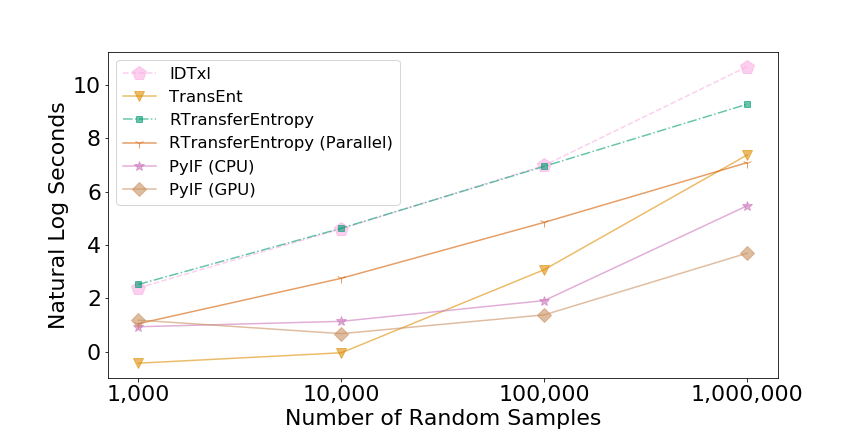
\includegraphics[scale=0.8]{figures/PyIF/WallTime-TE.png}}
  \caption{This figure shows the natural log time (in seconds) to estimate Transfer Entropy for each implementation (excluding Transfer Entropy Toolbox) for each dataset used in this study. }
  \label{TE-walltime}
\end{sidewaysfigure}


\begin{sidewaysfigure}[htb!]
  \centerline{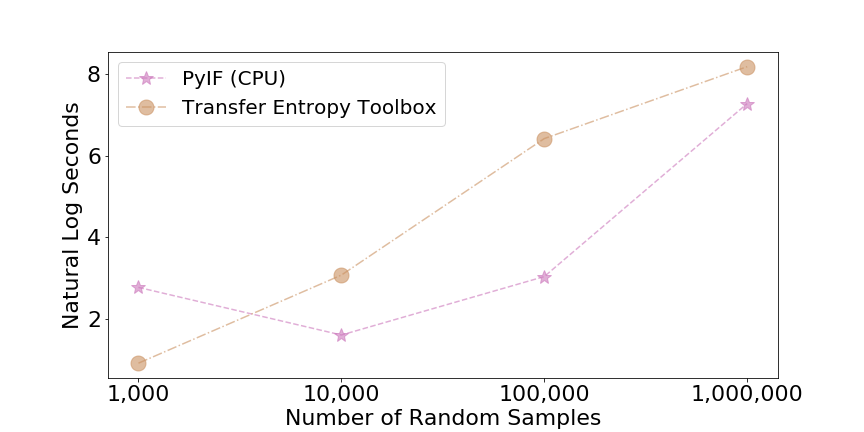
\includegraphics[scale=0.8]{figures/PyIF/WallTime-TE2.png}}
  \caption{This figure shows the natural log time (in seconds) to estimate Transfer Entropy between PyIF and Transfer Entropy Toolbox on an Engineering Workstation described in the Comparative Analysis section. Transfer Entropy Toolbox exceeded the maximum allowable CPU runtime for the Large Dataset. (1,000,000 observations). }
  \label{TE-walltime2}
\end{sidewaysfigure}

\clearpage

%\section*{Tables}

\begin{table}[htb!]
\centering
\resizebox{\columnwidth}{!}{
\begin{tabular}{|c|c|c|}
\hline
\textbf{Implementation}     & \textbf{Wall Time (in seconds)} & \textbf{Relative Performance to PyIF (CPU)} \\ \hline
IDTxl                       & 10.98                           & 4.28                                        \\ \hline
TransEnt                    & 0.656                           & 0.25                                        \\ \hline
RTransferEntropy            & 12.492                          & 4.87                                        \\ \hline
RTransferEntropy (Parallel) & 2.876                           & 1.12                                        \\ \hline
PyIF (CPU)                  & 2.564                           & 1                                           \\ \hline
PyIF (GPU)                  & 3.282                           & 1.28                \\ \hline                       
\end{tabular}
}
\caption{Micro Data results for the first analysis.}
\label{tab:MicroResults1}
\end{table}

\begin{table}[htb!]
\centering
\resizebox{\columnwidth}{!}{
\begin{tabular}{|c|c|c|} 
\hline
\textbf{Implementation}     & \textbf{Wall Time (in seconds)} & \textbf{Relative Performance to PyIF (CPU)} \\ \hline
IDTxl                       & 100.23                          & 31.94                                       \\ \hline
TransEnt                    & 0.968                           & 0.308                                       \\ \hline
RTransferEntropy            & 102.228                         & 32.57                                       \\ \hline
RTransferEntropy (Parallel) & 15.703                          & 5                                           \\ \hline
PyIF (CPU)                  & 3.138                           & 1                                           \\ \hline
PyIF (GPU)                  & 1.98                            & 0.63                                       \\ \hline
\end{tabular}
}
\caption{Small Data results for the first analysis.}
\label{tab:SmallResults1}
\end{table}

\begin{table}[htb!]
\centering
\resizebox{\columnwidth}{!}{
\begin{tabular}{|c|c|c|}
\hline
\textbf{Implementation}     & \textbf{Wall Time (in seconds)} & \textbf{Relative Performance to PyIF (CPU)} \\
IDTxl                       & 1070.749                        & 152.89                                      \\ \hline
TransEnt                    & 21.708                          & 3.03                                        \\ \hline
RTransferEntropy            & 1036.661                        & 152                                         \\ \hline
RTransferEntropy (Parallel) & 127.281                         & 18.66                                       \\ \hline
PyIF (CPU)                  & 6.82                            & 1                                           \\ \hline
PyIF (GPU)                  & 3.996                           & 0.58                      \\ \hline                 
\end{tabular}
}
\caption{Medium Data results for the first analysis.}
\label{tab:MediumResults1}
\end{table}

\begin{table}[htb!]
\centering
\resizebox{\columnwidth}{!}{
\begin{tabular}{|c|c|c|}
\hline
\textbf{Implementation}     & \textbf{Wall Time (in seconds)} & \textbf{Relative Performance to PyIF (CPU)} \\ \hline
IDTxl                       & 43150.129                       & 181.97                                      \\ \hline
TransEnt                    & 1585.942                        & 6.68                                        \\ \hline
RTransferEntropy            & 10592.77                        & 44.67                                       \\ \hline
RTransferEntropy (Parallel) & 1188.636                        & 5.01                                        \\ \hline
PyIF (CPU)                  & 237.122                         & 1                                           \\ \hline
PyIF (GPU)                  & 40.231                          & 0.16                                    \\ \hline   
\end{tabular}
}
\caption{Large Data results for the first analysis.}
\label{tab:LargeResults1}
\end{table}



% ake seperate table
\begin{table}[htb!]
\centering
\resizebox{\columnwidth}{!}{
		\begin{tabular}{ |c|c|c|  }
			\hline
			Implementation & Wall Time (in seconds) &  Relative Performance to PyIF (CPU) \\
 			\hline
			 \multicolumn{3}{|c|}{Micro Dataset Results (1000 Obs.)} \\
 			\hline
 			PyIF (CPU)   & 16.049 & 1.00\\ \hline
 			Transfer Entropy Toolbox & 2.5012 & 0.15 \\ \hline
 			\multicolumn{3}{|c|}{Small Dataset Results (10,000 Obs.)} \\ \hline
 			PyIF (CPU)   & 4.989 & 1.00\\ \hline
			 Transfer Entropy Toolbox & 21.6880 & 4.347 \\ \hline
 			\multicolumn{3}{|c|}{Medium Dataset Results (100,000 Obs.)} \\
 			\hline
 			PyIF (CPU)   & 20.915 & 1.00\\ \hline
			Transfer Entropy Toolbox & 616.8712 & 29.49 \\ \hline
 			\multicolumn{3}{|c|}{Large Dataset Results (1,00,000 Obs.)} \\
 			\hline
 			PyIF (CPU)   & 1455.725 & 1.00\\ \hline
			 Transfer Entropy Toolbox & $>$ 3600 & $>$ 2.47\\ 
			 \hline
			 

		\end{tabular}
	}
		\caption{Results for the second analysis.}
		%\caption{The wall time and relative performance to PyIF (CPU) to estimate Transfer Entropy between PyIF and Transfer Entropy Toolbox on an Engineering Workstation machine as described in the section Comparative Analysis.}
	\label{DataTable-MATLAB}
	
\end{table}

%\clearpage
\bibliographystyle{plainnat}
\nobibliography{thesisbib}